\chapter{Introduction}

\section{Motivation}
In recent years, English has been more commonly the preferred language of communications in many setting. The assessment of spoken English has therefore become increasingly important, especially in the context of education and employment opportunities. Traditionally, human examiners have been used to evaluate spoken English, but this approach is time-consuming and subjective. As a result, there has been a growing interest in developing automated systems for spoken language assessment.

Multiple systems have been developed to examine the spoken language proficiency of candidates. Three commonly investigated systems are text-based, feature-based, and speech-based systems \cite{graders}. Each type of model has its own method of processing the input speech and generating the intermediate vector $\mathbf{\hat{x}}$ (Chapter \ref{chap:graders}), which encapsulates information about the speech. Vector $\mathbf{\hat{x}}$ is passed into different neural network graders to produce the final score. The scoring process within the neural network is hard to be interpreted, causing non-transparency in the grading process. Problems such as potential biases within the system may then go undetected.

\begin{figure}[H]
    \centering
    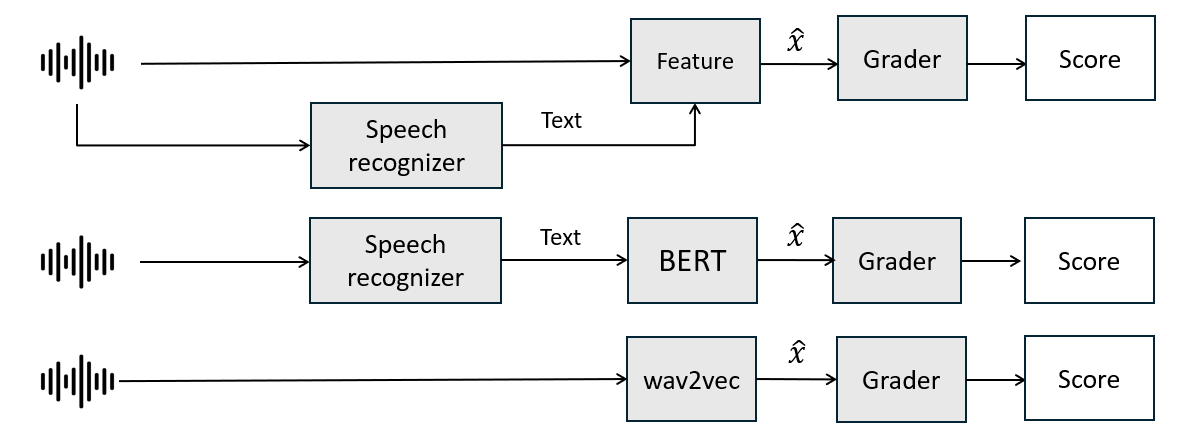
\includegraphics[width=0.7\textwidth]{grader.png}
    \caption{Spoken language assessment system for determining scores under consideration}
    \label{grader}
\end{figure}

A grader is unbiased if it evaluates speech samples solely based on performance-related factors, such as vocabulary richness and fluency, without being influenced by irrelevant attributes like gender, age and first language. It is important to ensure that the grading process is fair for candidates of all background, as unfair evaluations could have serious consequences for candidates' academic and professional opportunities. However, biases have previously been detected in other language models. For example, as existing natural language processing (NLP) tool are mainly trained with standard American English, language identifier misclassifies more frequently when processing African-American English as other languages, leading to biased results \cite{bias}. It is reasonable to expect that similar biases may exist in the spoken language assessment systems, performing particularly poorly for specific groups of candidates. Hence, it is pivotal to develop rigorous methods to measure and mitigate bias in these systems.

\section{Previous Work}
Concept activation vector (CAV) \nomenclature[Z]{CAV}{Concept Activation Vector} has previously been used to measure bias in a feature-based deep density network (DDN) \nomenclature[Z]{DDN}{Deep Density Network} models \cite{feature_bias}. Features related to the audio (energy level) and fluency (silence duration, long silence duration, word number and frequency, phone duration) are extracted from the audio as the intermediate vector \cite{feature_vector_old}. The CAV is extracted from the neural network without using weighting. There are two methods for CAV to measure bias: gradient-based (Chapter \ref{chap:cav}) and feature-based distance. The previous work investigated both methods.

% The experiment involves candidate data from the Use of Business English test (BULATS), which involves an initial short answer section, a read-aloud section, and three more general free speaking prompt-response answers. The scores were averaged over all sections to yield a score in the range 0 to 6.

When CAV indicated the presence of bias, the model's performance for that group of candidates, measured by the root mean squared error (RMSE), \nomenclature[Z]{RMSE}{Root Mean Squared Error} may or may not be worse than the initial performance. However, when CAV indicated the absence of bias for a particular group of candidates, the model's performance for them are also as good as the overall performance. This mean the CAV might not be sufficient to indicate bias presence, but enough to indicate the absence of it.

\section{Approach}
While the previous focuses on feature-based model, there are other types of models, which takes in text and speech, rather than features, as the input. The performance of CAV on these types of models is not well understood. The work aims at extending the investigation of CAV to other types of models. The gradient distance method is focused on, and it is found that the models display different gradient distance pattern.

In addition, previous research did not take into account the imbalance of concepts in the dataset, which could affect the CAV performance. Dataset might have more negative concepts than positive concepts. For example, people with their first language (L1) \nomenclature[Z]{L1}{First Language} as Thai is far less than people having other L1. The CAV extraction would not try to weight the minority group higher. Hence, the effect of using balanced weighting in the CAV extraction process is explored. It is shown that despite a difference in CAV performance, the ability of measuring bias is not affected.

The different types of models differ in terms of the input they take, and the design of the neural network grader. The work therefore attempts to isolate the factors affecting the difference in bias measurement across the models. The input into the system is found to be the factor having the most significant impact on the gradient distance pattern.

\section{Report Outline}
This report consists of 6 chapters with the following structure:
\begin{itemize}
    \item Chapter \ref{chap:graders} describes the different types of graders which would have its fairness being measured.
    \item Chapter \ref{chap:cav} outlines the steps of CAV extraction.
    \item Chapter \ref{chap:setup} describes the construction of training, calibration and testing data, alongside explanation on model biasing, factor isolation setup, and justification of performance metrics and hyper-parameters.
    \item Chapter \ref{chap:results} presents the results of the experiment, and discusses the implications.
    \item Chapter \ref{chap:conclusions} concludes the report and discusses future work.
\end{itemize}